\chapter{Attack and Loss Event}

\begin{figure}[H]
\centering
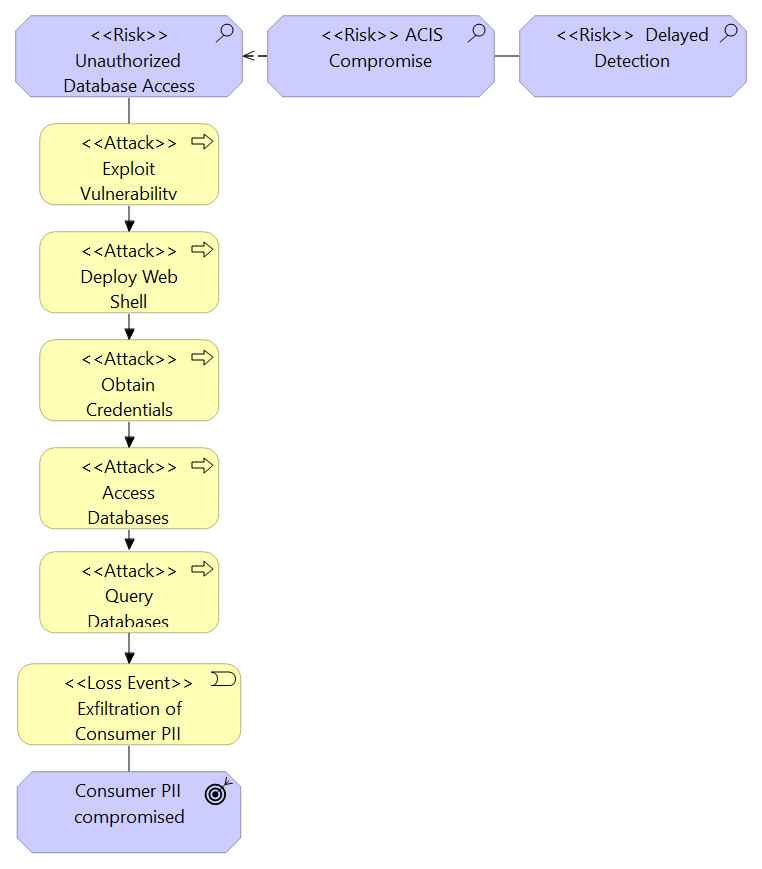
\includegraphics[width=0.5\linewidth]{images/attack-loss-view.png}
\caption{Attack \& loss view.}
\end{figure}

The given view shows the transition from the identified threats, vulnerabilities, risks and affected assets to the actual incident. It is modeled as the sequence of the incident, starting from the unauthorized database access and the related ACIS compromise and its delayed detection.
\newline
The sequence starts when the attackers exploit the vulnerability found in ACIS. There, they deployed a web shell to gain remote access to the compromised environment.
\newline
After ACIS was initially compromised, they obtained a file containing unencrypted credentials needed to access the databases inside the Equifax network.
\newline
From there, they started to perfom up to 9.000 queries to the databases in search of valuable information.
\newline
The sequence ends with the attackers obtaining consumer's PII in the databases and subsequently, exfiltrating them, leaving them compromised.